\documentclass[reprint,english,notitlepage,aps,nobalancelastpage,nofootinbib]{revtex4-1}
\usepackage[utf8]{inputenc}
\usepackage[english]{babel}
\usepackage{physics,amssymb}
\usepackage{graphicx}
\usepackage{xcolor}
\usepackage{hyperref}
\usepackage{tikz}
\usepackage{listings}
\usepackage{subfigure}
\usepackage{amsmath,mathtools}
\usepackage{amsbsy}
\usepackage{enumitem}
\usepackage{bbold}

\graphicspath{{../plots/}}

\hypersetup{
    colorlinks,
    linkcolor={red!50!black},
    citecolor={blue!50!black},
    urlcolor={blue!80!black}}

\lstset{
	inputpath=,
	backgroundcolor=\color{white!88!black},
	basicstyle={\ttfamily\scriptsize},
	commentstyle=\color{magenta},
	language=Python,
	morekeywords={True,False},
	tabsize=4,
	stringstyle=\color{green!55!black},
	frame=single,
	keywordstyle=\color{blue},
	showstringspaces=false,
	columns=fullflexible,
	keepspaces=true}


\makeatletter 

\renewcommand\onecolumngrid{% <<<<<<
\do@columngrid{one}{\@ne}%
\def\set@footnotewidth{\onecolumngrid}% <<<<<<<<<<<<<<<<
\def\footnoterule{\kern-6pt\hrule width 1.5in\kern6pt}%
}

\renewcommand\twocolumngrid{% <<<<<<
		\def\footnoterule{% restore rule
		\dimen@\skip\footins\divide\dimen@\thr@@
		\kern-\dimen@\hrule width.5in\kern\dimen@}
		\do@columngrid{mlt}{\tw@}
}%

\makeatother   

\newcommand{\closed}[1]{\left(#1\right)}
\newcommand{\bracket}[1]{\left[#1\right]}

\newcommand{\tmdv}[4]{\closed{\pdv{#1}{#2}}_{#3,#4}}
\newcommand{\jacobian}[2]{\pdv{(#1)}{(#2)}}
\renewcommand{\d}{\mathrm{d}}
\newcommand{\sumstate}{\sum_{\{\sigma_j\}}}
\newcommand{\prodstate}{\prod_{i=0}^{L-1}}
\newcommand{\ebj}{e^{\beta J}}
\newcommand{\T}[1]{T_{\sigma_{#1},\sigma_{#1 + 1}}}
\renewcommand{\l}{\lambda}
\newcommand{\mj}{m_j}
\newcommand{\tj}{T/J}

\begin{document}
\begin{center}
\title{\Huge FYS4130 - Oblig 2}
\author{\large Vetle A. Vikenes}
\date{\today}
\noaffiliation


\maketitle
\end{center}


\onecolumngrid


\section*{\large Task 1 - Transfer Matrices}

\subsection*{a) Partition function and average internal energy}

We consider a 1D spin chain of length $L$ with periodic boundary conditions. The Hamiltonian of the system given as  
\begin{align} \label{eq:Hamiltonian}
	H &= -J \sum_{i=0}^{L-1} \delta_{\sigma_i,\sigma_{i+1}},
\end{align}

where $\sigma_i=\{0,\,1,\,2\}$ denotes the spin at site $i$ and $J>0$.    

The order parameter, $m$, and local magnetization, $m_j$, is given by
\begin{align}
	m &\equiv \frac{1}{N} \sum_{j=0}^{N-1} m_j \label{eq:order parameter}  \\ 
	\text{where}\quad m_j &\equiv e^{i(2\pi/3)\sigma_j} \label{eq:magnetization}
\end{align}

To calculate the partition function, we begin by inserting the expression for the Hamiltonian and write the sum in the exponent in terms of products. 
\begin{align*}
	Z &= \sum_{\{\sigma_j\}} e^{-\beta H} = \sumstate e^{\beta J \sum_{i=0}^{L-1} \delta_{\sigma_i,\sigma_{i+1}}} = \sumstate \prod_{i=0}^{L-1} e^{\beta J \delta_{\sigma_i,\sigma_{i+1}}}
\end{align*}

The exponential can be written in terms of transfer matrices representing the different values of the exponential for different spin states. Letting $\sigma_i$ and $\sigma_{i+1}$ govern the row and column, respectively, the transfer matrix becomes 

\begin{align} \label{eq:transfer_matrix}
	T_{\sigma_i,\sigma_{i+1}} &= 
	\begin{pmatrix}
		e^{\beta J} & 1 & 1 \\
		1 & \ebj & 1 \\
		1 & 1 & \ebj
	\end{pmatrix}.
\end{align}

The transfer matrix will thus look identical for different values of $\sigma_i$, so taking the product between different ones, results in a transfer matrix raised to a certain power.  

\begin{align*}
	Z &= \sumstate \prodstate \T{j} = \sumstate T_{\sigma_0,\sigma_1} T_{\sigma_1,\sigma_2}\cdots T_{\sigma_{L-1},\sigma_0} 
\end{align*}
where we invoked the periodicity, $\sigma_L=\sigma_0$, in the last line. This means that we're summing over repeated indices, and the sum can be carried out by taking the trace of the resulting matrix products. To calculate the product of the matrices, we start by diagonalizing it, writing it as $T=PDP^{-1}$, with

\begin{align*}
	P &= 
	\begin{pmatrix*}[r]
		-1 & -1 & 1 \\ 
		0  & 1  & 1 \\ 
		1  & 0  & 1 
	\end{pmatrix*} ,\quad D = \begin{pmatrix*}[r]
		\lambda_1 & 0 & 0 \\ 
		0 & \lambda_2 & 0 \\
		0 & 0 & \lambda_3 
	\end{pmatrix*},\quad
	P^{-1} = \frac{1}{3} \begin{pmatrix*}[r]
		-1 & -1 & 2 \\ 
		-1 & 2  & -1 \\ 
		1  & 1  & 1
	\end{pmatrix*},
\end{align*}

where the eigenvalues of $T$ are 
\begin{align*}
	\lambda_1 &= \ebj-1 \\ 
	\lambda_2 &= \ebj-1 \\ 
	\lambda_3 &= \ebj+2
\end{align*}

Since the summation of transfer matrices in our expression for $Z$ is over repeated indices, the sum corresponds to taking the trace of the matrix, so our expression for $Z$ becomes 

\begin{align*}
	Z &= \Tr(T_{\sigma_0,\sigma_0}^N) = \Tr(PDP^{-1}PDP^{-1}\cdots PDP^{-1}) \\ 
	&=Tr(P D^L P^{-1})= \Tr(D^L) = \lambda_1^L + \lambda_2^L + \lambda_3^L,
\end{align*}
where we used the cyclic property of the trace to eliminate the final $P$ and $P^{-1}$. 

Inserting the eigenvalues, we finally arrive at 
\begin{align}
	Z &= 2\closed{\ebj - 1}^L + \closed{\ebj+2}^L \label{eq:partition_function}
\end{align}

We will now use equation \eqref{eq:partition_function} to calculate the average total energy, $U$, which is obtained through the following partial derivative  

\begin{align*}
	U &= \pdv{(\beta F)}{\beta}.
\end{align*}

The product $\beta F$ is gotten from the negative logarithm of $Z$, and is thus 

\begin{align*}
	\beta F = -\ln Z = -\ln\bracket{2(\ebj-1)^L + (\ebj+2)^L}.
\end{align*}

Differentiating this with respect to $\beta$, we get

\begin{align}
	U &= -\frac{2L(\ebj-1)^{L-1} J\ebj + L(\ebj+2)^{L-1}J\ebj}{2(\ebj-1)^L + (\ebj+2)^L} \nonumber \\[10pt]
	& = -LJ\ebj \cdot \frac{2(\ebj-1)^{L-1}+(\ebj+2)^{L-1}}{2(\ebj-1)^L + (\ebj+2)^L} \label{eq:avg_tot_en}
\end{align}

Now, we want to find an approximate expression for $U$ valid for low and high temperatures. Rather than working with $U$ directly, we will instead rewrite the partition function in a way that allows us to simplify it. 
\begin{align*}
	Z = 2\l_1^L + \l_3^L = \l_3^L\bracket{2\closed{\frac{\l_1}{\l_3}}^L+1},
\end{align*} 
where a factor $\l_3$ has been taken outside the brackets, since $\l_3>\l_1$. For large values of $L$ we can now see that the behaviour of $Z$ is restricted to two separate cases, corresponding to small and large values of $\beta$. 

If $\beta$ is very large, the constant terms of the eigenvalues become negligible, so we get $\l_1/\l_3\approx1$. In this case we get $Z\approx 3\l_3^L$. If, on the other hand, $\beta$ is small we have $\l_1\ll \l_3 \implies (\l_1/\l_3)^L \to 0$. The expression for $Z$ is then $Z\approx \l_3^L$.  

Our two expressions for $Z$ differs only by a constant factor. Upon differentating the logarithm of $Z$ this constant vanishes, so our approximate expression for $U$ becomes       
\begin{align*}
	U&=-\pdv{\beta}\ln Z \approx -\pdv{\beta} L \ln \l_3 = -L \pdv{\beta}\ln (\ebj+2) \\ 
	&= -\frac{LJ}{1+2 e^{-\beta J}}, 
\end{align*}
which is valid at both high and low values of $T$. Computing the two limiting cases, we find  

\begin{align*}
	\lim_{\beta\to\infty} U = -LJ,\:\:\text{and}\quad \lim_{\beta\to0} U = -\frac{LJ}{3}
\end{align*}
Using WolframAlpha, we get the same results for the two limits of $U$ from equation \eqref{eq:avg_tot_en}, and therefore conclude that our approximation is reasonable. 

For the physical interpretation, the low temperature limit corresponds to our model having its minimum energy, where all the spins are aligned. In the high temperature limit we have disordered spin states, uniformly distributed among the three possible values of $\sigma_j$. The probability of neighbouring spins being aligned in this case is then $1/3$, such that the Hamiltonian only yields a non-zero term in its sum for $1/3$ of all the configurations.


\subsection*{b) - Average magnetization}

We now want to show that the average magnetization, $\expval{m}$, equals zero at all temperatures. We can express the average magnetization as 
\begin{align*}
	\expval{m} = \frac{1}{N} \sum_{i=0}^{N-1}\expval{m_j},
\end{align*}
and we can now compute $\expval{\mj}$, and we start by inserting transfer matrices, as we did before.  

\begin{align*}
	\expval{m_j} &= \frac{1}{Z} \sumstate \mj e^{-\beta H} = \frac{1}{Z} \sumstate e^{i(2\pi/3)\sigma_j} \prodstate \T{j}
\end{align*} 

Summing all the spins from $\sigma_1$ up to $\sigma_{j-1}$ yields a factor of $T_{\sigma_0,\sigma_j}^j$ at the beginning as well as a similar factor raised to the power $L-j$ at the end, so $\expval{\mj}$ can therefore be written as   

\begin{align*} 
	\expval{\mj} &= \frac{1}{Z} \sum_{\sigma_0} \sum_{\sigma_j} T_{\sigma_0,\sigma_j}^j e^{i(2\pi/3)\sigma_j} \,T_{\sigma_j,\sigma_0}^{L-j}
\end{align*}
To carry out the sum, we now use that we sum over repeated indices and we thus have to compute the trace of the resulting matrix. Since the diagonal elements of the original transfer matrix in equation \eqref{eq:transfer_matrix} are identical, the diagonal elements of the same matrix raised to a certain power will also be identical. This leaves us with the same factor in front of the three different exponential terms, and we get 

\begin{align*}
	\expval{\mj} &= \frac{1}{Z} \closed{T_{0,0}^j\,T_{0,0}^{L-j} + e^{i2\pi/3} \,T_{1,1}^j\,T_{1,1}^{L-j} + e^{-i2\pi/3}\,T_{2,2}^j\,T_{2,2}^{L-j}} \\ 
	&= \frac{1}{Z} \closed{1 + e^{i2\pi/3} + e^{-i2\pi/3}} 3\,T_{0,0}^{j} \, T_{0,0}^{L-j} \\ 
	&= 0.
\end{align*}  
With $\expval{\mj}=0$ we then get $\expval{m}=\sum \expval{\mj}/N=0$, which is what we wanted to show.


\subsection*{c) - Correlation function}
The correlation function is defined as 
\begin{align} \label{eq:corr_func}
	C(r) &\equiv \expval{m_0^* m_r} - \expval{m_0^*}\expval{m_r}.
\end{align}
Having already found that $\expval{\mj}=0$, the last term in equation \eqref{eq:corr_func} vanishes, and we're left with the quantity $\expval{m_0^* m_r}$, which we can write in terms of exponentials as 

\begin{align*}
	\expval{m_0^* m_r} &= \expval{e^{i(2\pi/3)(\sigma_r - \sigma_0)}}.
\end{align*}

We follow the same procedure as before, writing out all sums except for the ones over $\sigma_0$ and $\sigma_r$ this time. 

\begin{align*}
	\expval{m_0^* m_r} &= \frac{1}{Z} \sumstate m_0^* m_r \, \prodstate \T{i} = \frac{1}{Z} \sum_{\sigma_0} \sum_{\sigma_r} e^{i\frac{2\pi}{3}(\sigma_r-\sigma_0)} T_{\sigma_0,\sigma_r}^{r} \, T_{\sigma_r,\sigma_0}^{L-r} 
\end{align*}

Now, the exponential term can be written as a matrix with indices $(\sigma_r,\sigma_0)$, meaning that we can't simply compute the trace in this case. Before computing anything, we will first consider the general form of the transfer matrices raised to a certain power. 

Using the diagonalization $T=PDP^{-1}$, we write the general expression for $T_{i,j}^k=(PD^k P^{-1})_{i,j}$ gotten from the matrix multiplication. The resulting matrix will have identical terms on the diagonal, as well as identical terms on the off-diagnoal. These terms are given in equation \eqref{eq:T_power}  

\begin{align} \label{eq:T_power}
	T_{i,j}^k = \frac{1}{3}\begin{cases}
		2(\ebj-1)^k + (\ebj+2)^k \quad &\mathrm{for}\; i=j \\ 
		-(\ebj-1)^k + (\ebj+2)^k \quad &\mathrm{for}\; i\neq j
	\end{cases}
\end{align}

When we sum over different spin combinations, there will be three terms corresponding the case of equal indices in equation \eqref{eq:T_power}, where the exponent simply contributes a factor $1$. On the off-diagonal, three terms will have a common factor of $e^{i(2\pi/3)}$. The same three terms will also have a common factor of $e^{-i(2\pi/3)}$, since $T_{i,j}=T_{j,i}$. For the off-diagonal terms we are then left with three terms having a common factor $e^{i(2\pi/3)} + e^{-i(2\pi/3)}=-1$. 

To simplify the writing, we write $T_{i=i}$ for diagonal terms and $T_{i\neq j}$ for off-diagonal terms.

\begin{align*}
	\expval{m_0^* m_r} =& \frac{1}{Z} \Big[ 3\, T_{i=i}^r T_{i=i}^{L-r} - 3T_{i\neq j}^r T_{i\neq j}^{L-r} \Big] \\ 
	=& \frac{3}{Z} \Bigg( \frac{1}{3} \Big[ 2(\ebj-1)^r + (\ebj+2)^r \Big]\cdot \frac{1}{3} \Big[2(\ebj-1)^{L-r} + (\ebj+2)^{L-r} \Big] \\ 
	&\quad\:\: -\frac{1}{3}\Big[(\ebj+2)^r-(\ebj-1)^r \Big] \cdot \frac{1}{3}\Big[(\ebj+2)^{L-r}-(\ebj-1)^{L-r} \Big]  \Bigg) \\
	=& \frac{1}{Z} \cdot \frac{1}{3} \Bigg( 4(\ebj-1)^L + (\ebj+2)^L + 2(\ebj-1)^r (\ebj+2)^{L-r} + 2 (\ebj+2)^r (\ebj-1)^{L-r}  \\
	& \qquad\quad - \Big[(\ebj-1)^L + (\ebj+2)^L - (\ebj-1)^r (\ebj+2)^{L-r} - (\ebj+2)^r (\ebj-1)^{L-r} \Big] \Bigg)
\end{align*}
The two terms $(\ebj+2)^L$ will now cancel each other out, while the remaining terms will all have a factor $3$ canceling the factor $1/3$ in front. Finally, writing out the partition function, our final expression for the correlation function becomes 

\begin{align} \label{eq:corr_func_result}
	C(r) &= \frac{(\ebj-1)^L + (\ebj-1)^r (\ebj+2)^{L-r} + (\ebj-1)^{L-r} (\ebj+2)^r}{2(\ebj-1)^L + (\ebj+2)^L}
\end{align}



Now we want to find the limiting result of $C(r)$ for $L\to\infty$. This is most easily done by resorting to WolframAlpha, from which we get that
\begin{align*}
	\lim_{L\to\infty} C(r) = \closed{\frac{\ebj-1}{\ebj+2}}^r = \closed{\frac{\l_1}{\l_3}}^r
\end{align*}
The limiting case is still a function of $r$, which is desired, since two spins separated by a short distance will still be correlated no matter how long the overall chain is. With $\l_1<\l_3$ we also get that the longer the separation between spins, the less they are correlated. 

For the case $T=0$, we let WolframAlpha compute the limit as $\beta\to\infty$ and get 
\begin{align*}
	\lim_{T\to0} C(r) = 1,
\end{align*}
implying that there is a perfect correlation between all spins. This coincides with the fact that all the spins are alligned when $T=0$, as discussed in 1a). 

\section*{\large Task 2 - Monte Carlo Simulations}

For simplicity, $k_B=J=1$ has been used in all calculation. 

\subsection*{a) - Monte carlo program}
The code that has been used in this task can be found on Github: \url{https://github.com/Vikenes/FYS4130/tree/main/oblig2/code}. The programs for computations are in the folder "cpp", while the python script is used for plotting. 

Having never written c++ before, my brain could not create a c++ algorithm suitable for both 1D and 2D within the deadline, so two separate scripts have been made. My inexperience will also be noticeable in places where I may have overlooked solutions that are obviously better/smarter than mine.    

\subsubsection*{Numerical parameters and detailed balance}

Unless stated otherwise, all of the Monte Carlo (MC) simulations have been run with $10^4$ number of equilibrium steps, and $10$ bins with $10^4$ measurement steps in each. Similarly, we use $L=16$ sites in each direction, unless stated otherwise, yielding $N=L$ for the 1D simulation and $N=L\cross L$ for the 2D simulation. 

When implementing the Wolff algorithm, we need to use a connection probability appropriate for the system we're considering. For a given spin on the ring, there is a probability $p$ of assigning a bond to one of its neighbours if it has the same spin. The probability of not including the neighbouring spin in the bond is then $1-p$. In both cases, the energy contribution from these spins are $\ebj$. For neighbouring sites with unequal spins, there is a probability of $1$ that we don't assign any bond, and the energy contribution from these sites are $e^0=1$. To get the correct probability for assigning spins to the cluster, we must fullfill the detailed balance, which in this case is the product of the energy between two spins and the probability that bonds are not assigned. The only situation where this factor changes when we flip spins, is when two neighbours initially have equal spins, but not a bond between them, and one of them is flipped. The detailed balance is then 
\begin{align}
	P(\text{equal spins, no bond})\cdot e^{\beta J} &= P(\text{unequal spins, no bond})\cdot e^{0} \nonumber  \\ 
	(1-p)\ebj &= 1 \nonumber \implies p = 1-e^{-\beta J} \\ 
	p &= 1 - e^{-1/T} \label{eq:connection_probability}
\end{align}      
where we in the last line used that $k_B=J=1$ in our simulations. 

\subsection*{b) - Correlation function}
We use the MC simulation to compute the three quantities needed to calculate the $C(r)$ as it is written in equation \eqref{eq:corr_func}. We plot this result against the analytical solution for both $\tj=0.25$ and $\tj=0.5$, shown in the upper and lower panel of figure \ref{fig:correlation} respectively


\begin{figure}[h!]
	\centering
	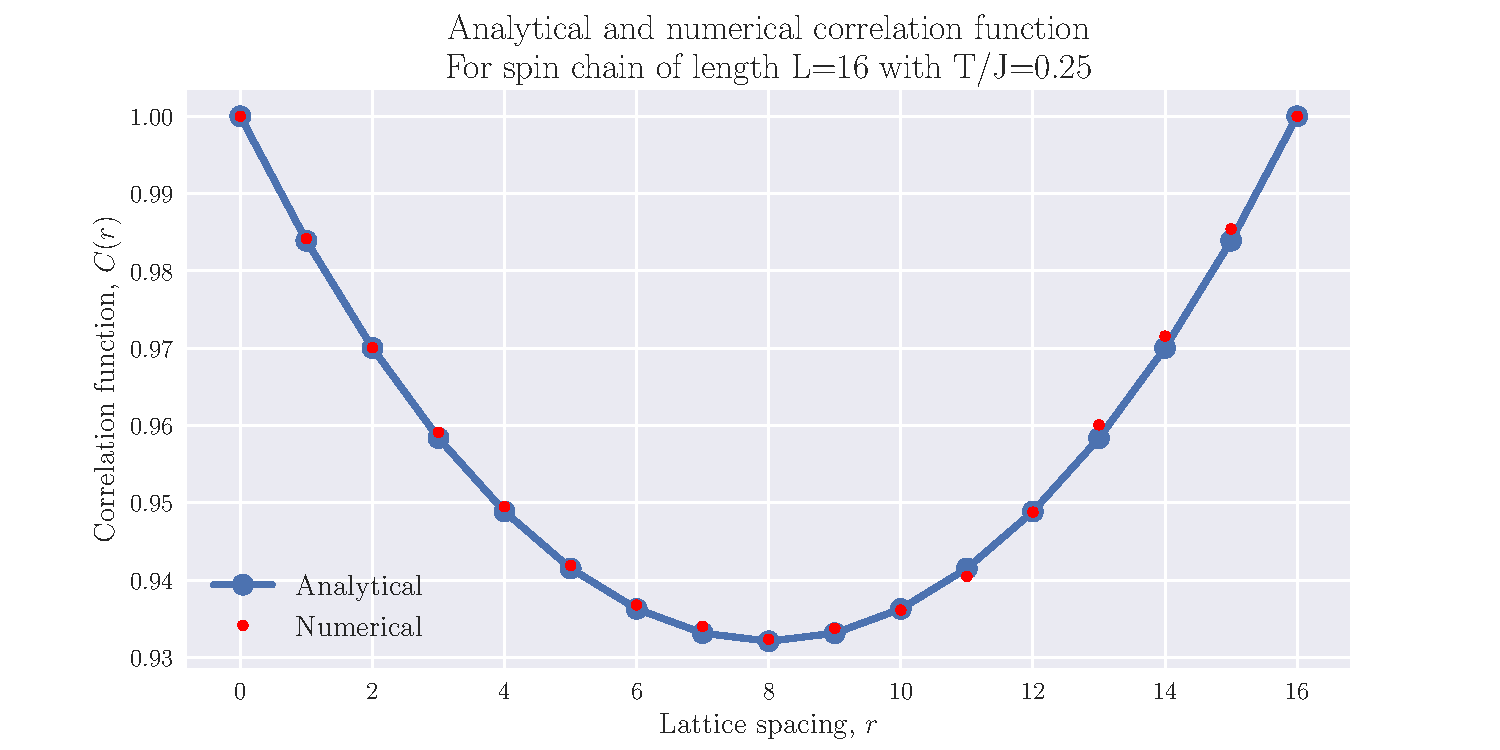
\includegraphics[width=0.8\linewidth]{correlation1D_025.pdf}
	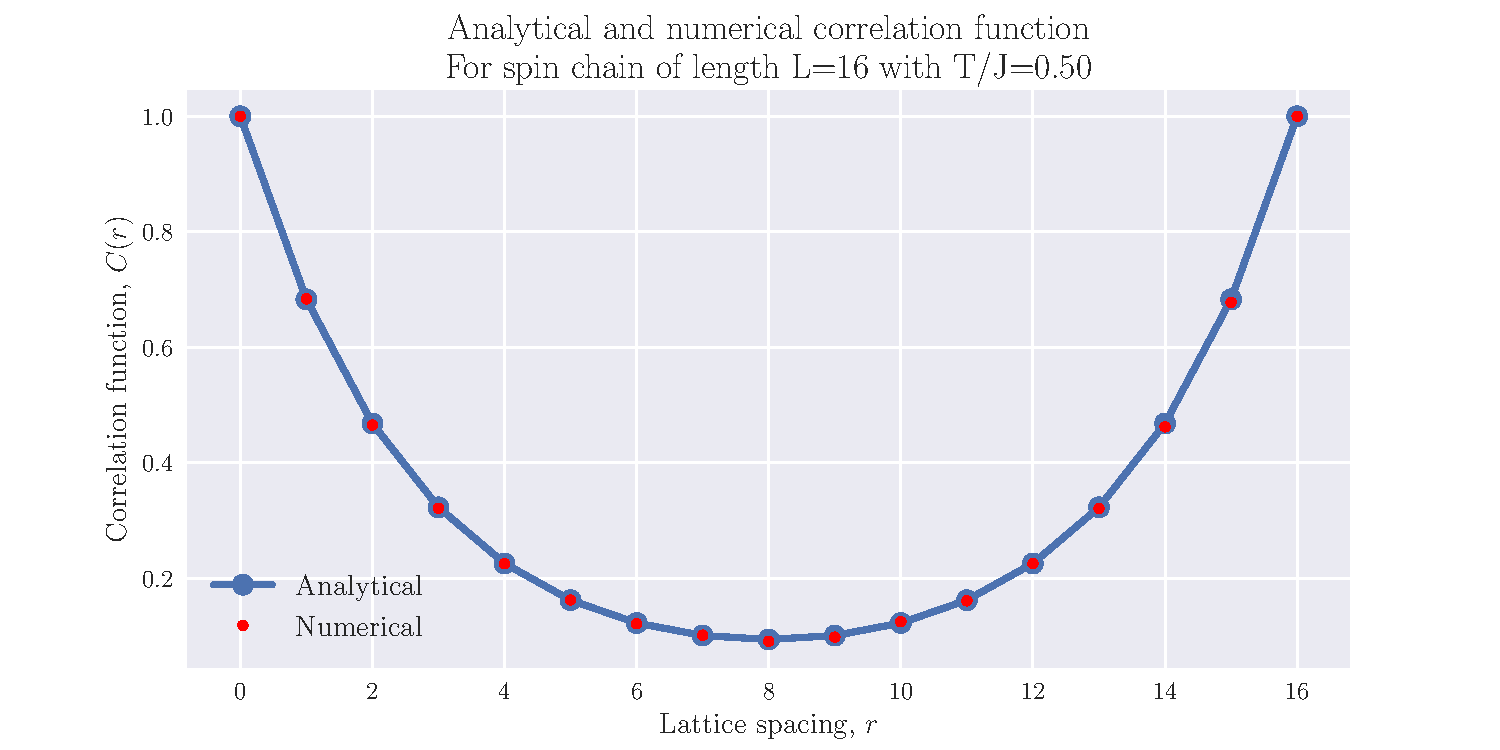
\includegraphics[width=0.8\linewidth]{correlation1D_05.pdf}
	\caption{Comparison between the numerically and analytically computed correlation function for the 1D spin chain at two different temperatures, using $\sigma_L=\sigma_0$.}
	\label{fig:correlation}
\end{figure}

For $\tj=0.5$, we see that the two correlation functions are overlapping nicely, while for $\tj=0.25$, there is some deviations between the two results. These deviations are most likely caused by the value of $p$ at low temperatures. Inserting the two temperature values in our expression for $p$ in equation \eqref{eq:connection_probability}, we get 
\begin{align*}
	p(T=0.5) &\approx 0.9817 \\ 
	p(T=0.25) &\approx 0.8647 
\end{align*} 
The high probability of assigning bonds when $T=0.25$ implies that we should attempt a new MC simulation with more steps, in order to get enough samples with bonds not being assigned. Using $10^5$ steps for equilibriation and measuremnts, as well as $20$ bins for the measurements, we compute $C(r)$ for $T=0.25$ once again, as shown in figure \ref{fig:correlation_incrN}. Now, the deviations are barely visible, and we conclude that our program works as it should \footnote{I realize that this doesn't guarantee that the 2D case works, as it is a separate script, but the basic structure of the two programs are unaltered and my results coincide with what other people have gotten}.

\begin{figure}[h!]
	\centering
	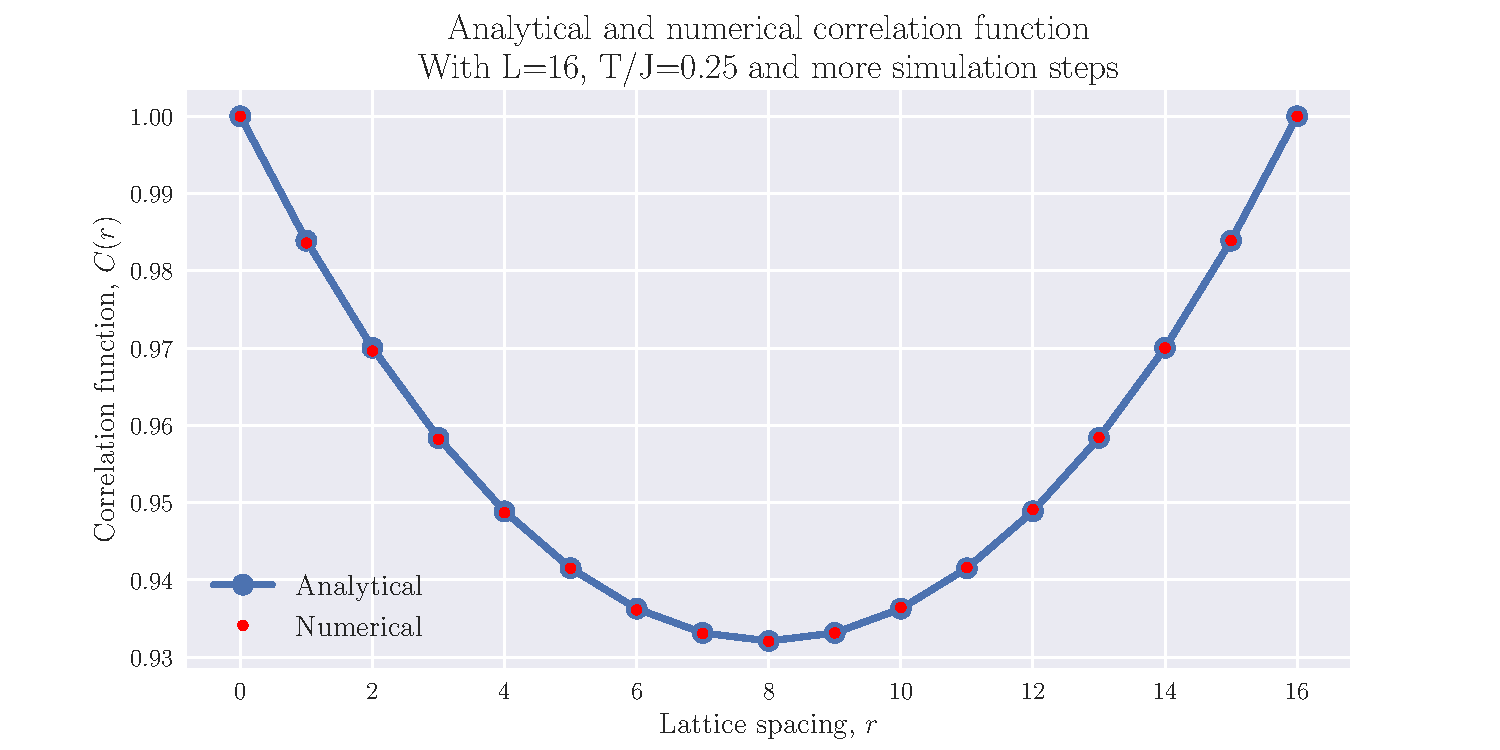
\includegraphics[width=0.7\linewidth]{correlation1D_025_incrN.pdf}
	\caption{Comparison of numerical and analytical correlation function with a factor $10$ increase of MC steps and twice the number of bins.}
	\label{fig:correlation_incrN}
\end{figure}

\subsection*{c) - Average magnetization}
Next, we plot the real part of the average magnetization $\expval{m}$ as a function of $\tj\in[0.1,\,10]$, shown in figure \ref{fig:avg_mag}. Included in the plot is the standard deviation $\sigma_N=1/\sqrt{N}$, due to finite measurements. We see that $\expval{m}$ is close to zero for low values of $\tj$, but fluctuates significantly as $\tj\to1$. For high values of $\tj$ we even get values of $\Re(\expval{m})\pm\sigma_N<0$, which we don't expect. At high $\tj$ values, the connection probability is fairly low, and we would expect that we got more stable values if we were to increase the number of MC steps.     

\begin{figure}[h!]
	\centering
	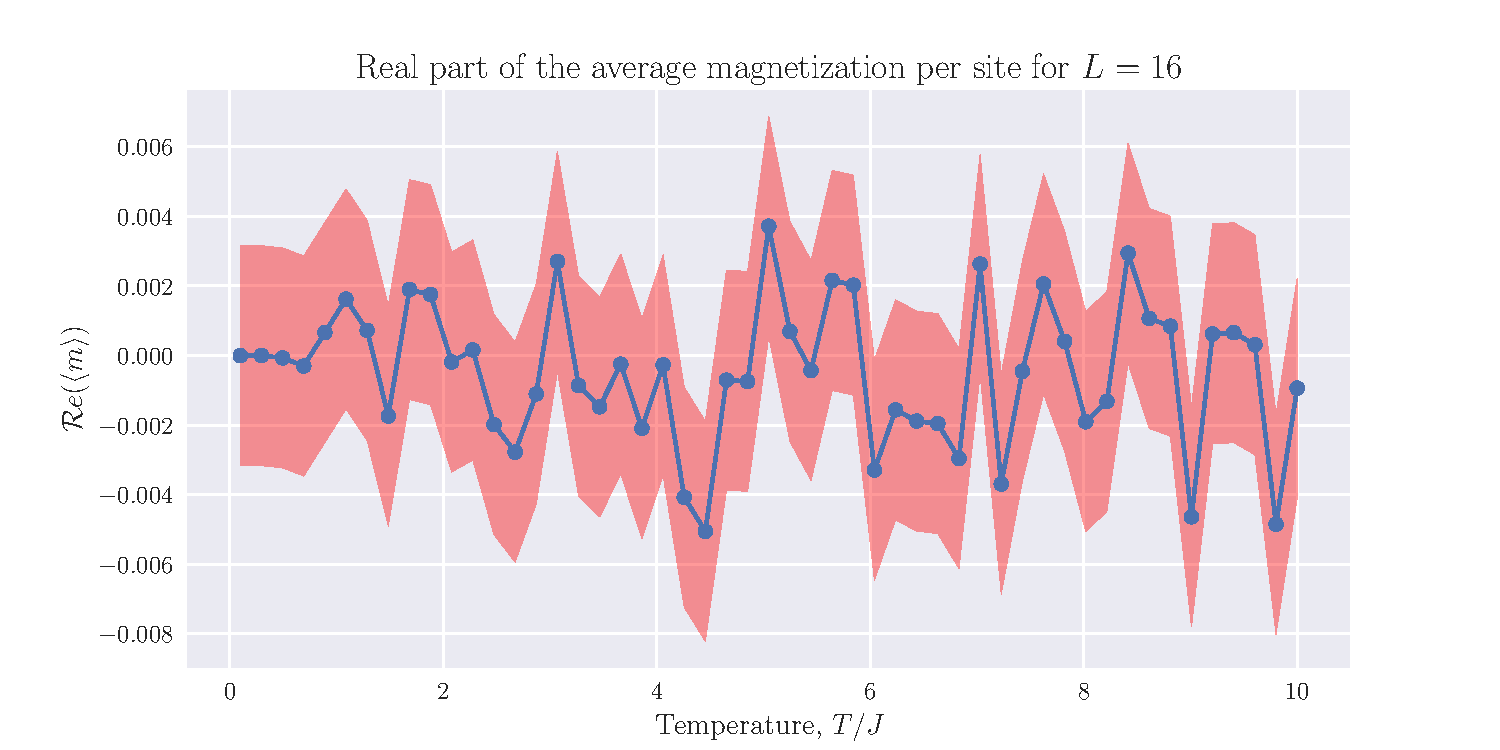
\includegraphics[width=0.7\linewidth]{avg_mag_re.pdf}
	\caption{Average magnetization for increasing temperatures, with standard deviations indicated by the shaded red area.}
	\label{fig:avg_mag}
\end{figure}

\subsection*{d) - Average magnetization squared}

The average magnetization squared per site, $\expval{\abs{m}^2}$ is plotted as a function of $\tj\in[0.01,\,2]$, shown in figure \ref{fig:avg_mag_squared}. We see that $\expval{\abs{m}^2}\to1$ as $\tj\to0$, while $\expval{\abs{m}^2}\to0$ as $\tj\to\infty$. At low $\tj$ the connection probability is very high, which favors alignment of spin. As previously discussed, we expect allignment of spins at low $T$. When spins are equal, taking the absolute value squared of one of the possible values of $m_j$ yields $1$. As $T$ increases, allignment of spins is no longer the case, so the overall average of spins are $0$.  

\begin{figure}[h!]
	\centering
	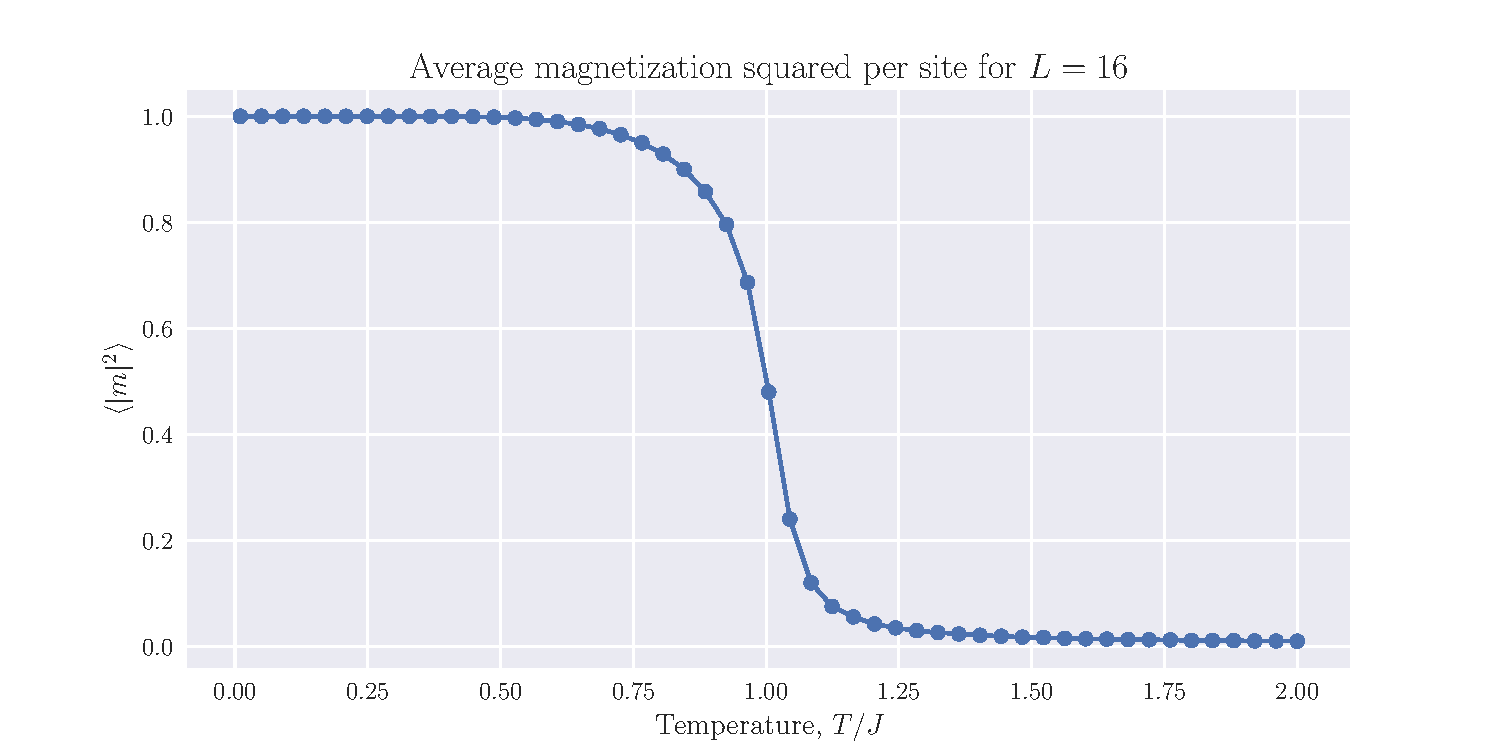
\includegraphics[width=0.7\linewidth]{avg_mag_squared.pdf}
	\caption{Average magnetization squared for increasing temperatures, showing the transition from ordered to disordered states.}
	\label{fig:avg_mag_squared}
\end{figure}

\subsection*{e) - Finite size scaling}

We want to show that curves of $\Gamma$ vs. $\tj$ crosses at the phase transition temperature for different values of $L$, where $\Gamma$ is defined as 
\begin{align*}
	\Gamma &\equiv \frac{\langle\abs{m}^4\rangle}{\langle\abs{m}^2\rangle ^2}
\end{align*}

We will assume that $\Gamma=\Gamma(t,L^{-1})$, where $t\equiv(T-T_c)/T_c$. We introduce dimensionless length, $L'^{-1}=(L/a)^{-1}$, where $a$ is the lattice spacing. Scaling the lattice spacing by a factor $s$, $a\to a'=sa$ makes the dimenionless length scale as $L'^{-1}\to sL'^{-1}$. Scaling $t$ and $L^{-1}$ by appropriate factors of $s$ yields the following scaling relation for $\Gamma$
\begin{align*}
	\Gamma(t,L^{-1}) &= s^0 \Gamma(t s^{y_t},\,L'^{-1} s)
\end{align*}

where $\Gamma$ itself is dimensionless, so it doesn't scaling with lattice spacing, and $y_t$ is the scaling exponent for $t$. We now choose $s=L'$, such that the finite scaling relation becomes 
\begin{align*}
	\Gamma(t,L^{-1}) = \Gamma(t L'^{y_t},1). 
\end{align*}   
We can now define the RHS to be $g(t L'^{y_t})$. Since $L'$ is finite, if we're close to the critical temperature we can expand $g$ around $t=0$
\begin{align*}
	g(t L'^{y_t}) = g(0) + t L'^{y_t} g'(0) + ... 
\end{align*}
Now, if are at the critical temperature, we have $t=0$, and the finite scaling relation becomes 
\begin{align*}
	\Gamma(t,L^{-1}) &= g(t L'^{y_t}) = g(0)
\end{align*}
and we see that RHS now has become independent of $L$. This means that for different choices of $L$, the resulting curves of $\Gamma$ should cross at the phase transition temperature. 

\subsection*{f) - Estimating the critical temperature}
We now plot $\Gamma$ as a function of $\tj\in[0.8,\,1.20]$ for the systems sizes $L=\{8,\,16,\,32\}$, using $50$ temperature points. Additionally we include a plot showing the crossing of the curves. These two plots as shown in the upper and lower panel of figure \ref{fig:gamma}, respectively.

\begin{figure}[h!]
	\centering
	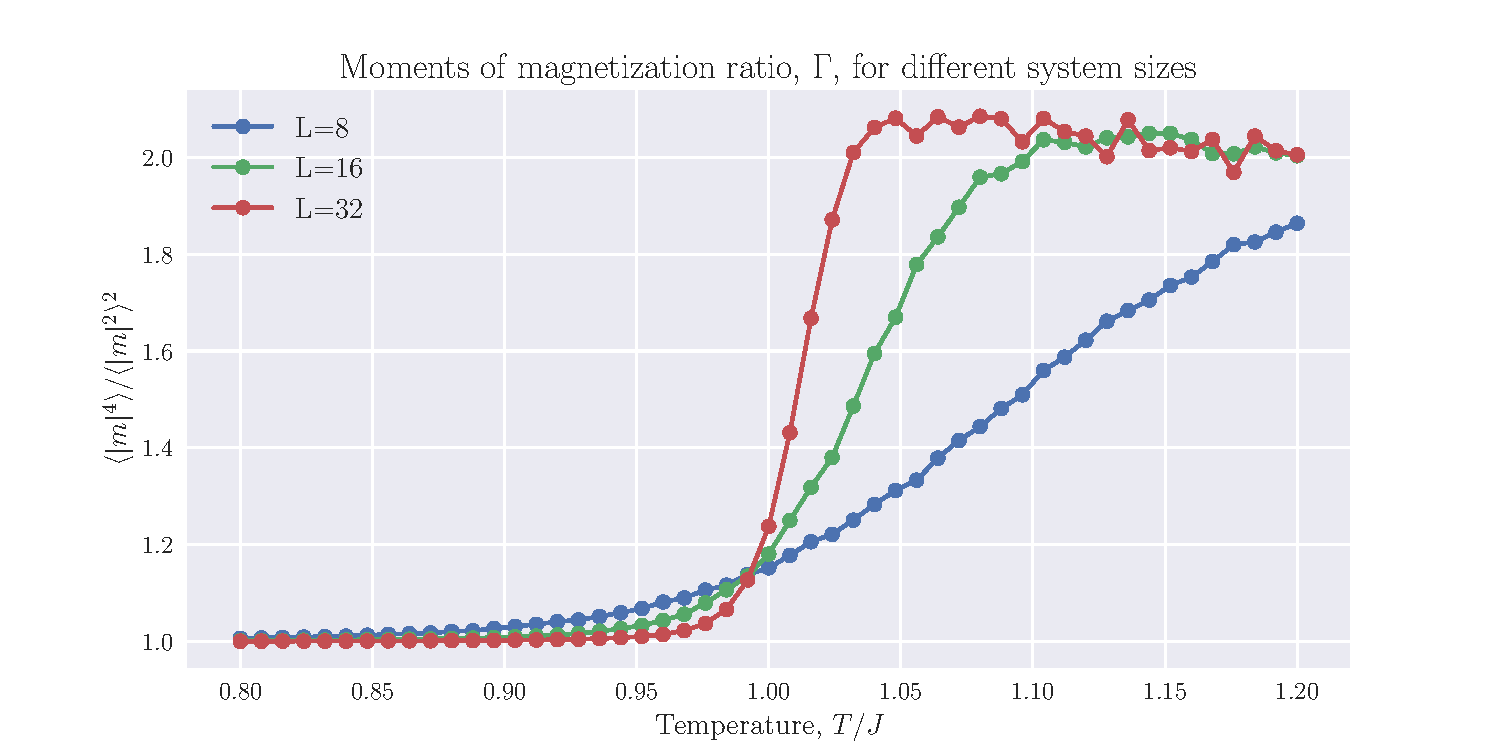
\includegraphics[width=0.7\linewidth]{gamma_curves_N51_dT04.pdf}
	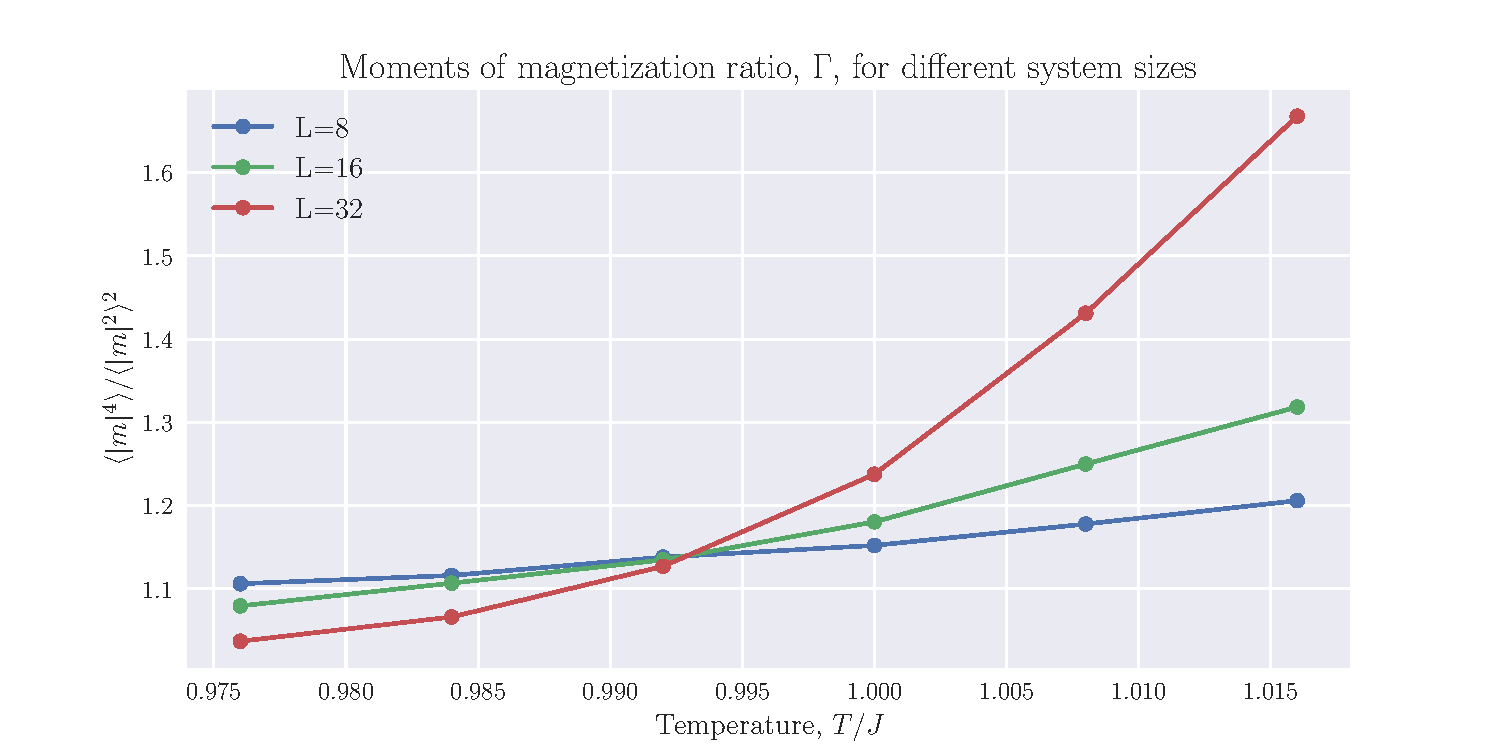
\includegraphics[width=0.7\linewidth]{gamma_curves_N6_dT004.pdf}
	\caption{Moments of magnetization for different system sizes. The crossing point indicates the critical temperature. In the lower panel we see that the curves don't overlap perfectly, but indicates that $0.99< T_c < 1$.}
	\label{fig:gamma}
\end{figure}
We see that the three curves appear to cross somewhere between $\tj=0.990$ and $\tj=0.995$, but we need a higher density of $\tj$ in this region to make a reasonable conclusion about the exact value of the critical temperature.

To investigate the crossing further, we use $50$ values of $\tj\in[0.99,\,1.00]$ and plot the resulting curves of $\Gamma$, shown in figure \ref{fig:gamma_dense}. The small temperature steps results in relatively large fluctuations of the $\Gamma$ curves, so we're still unable to conclude what $T_c/J$ is from this figure, but it appears to occur for $T<T_c$. For the sake of time we choose not to investigate the crossing point further with more MC simulation steps and more bins.   

\begin{figure}[h!]
	\centering
	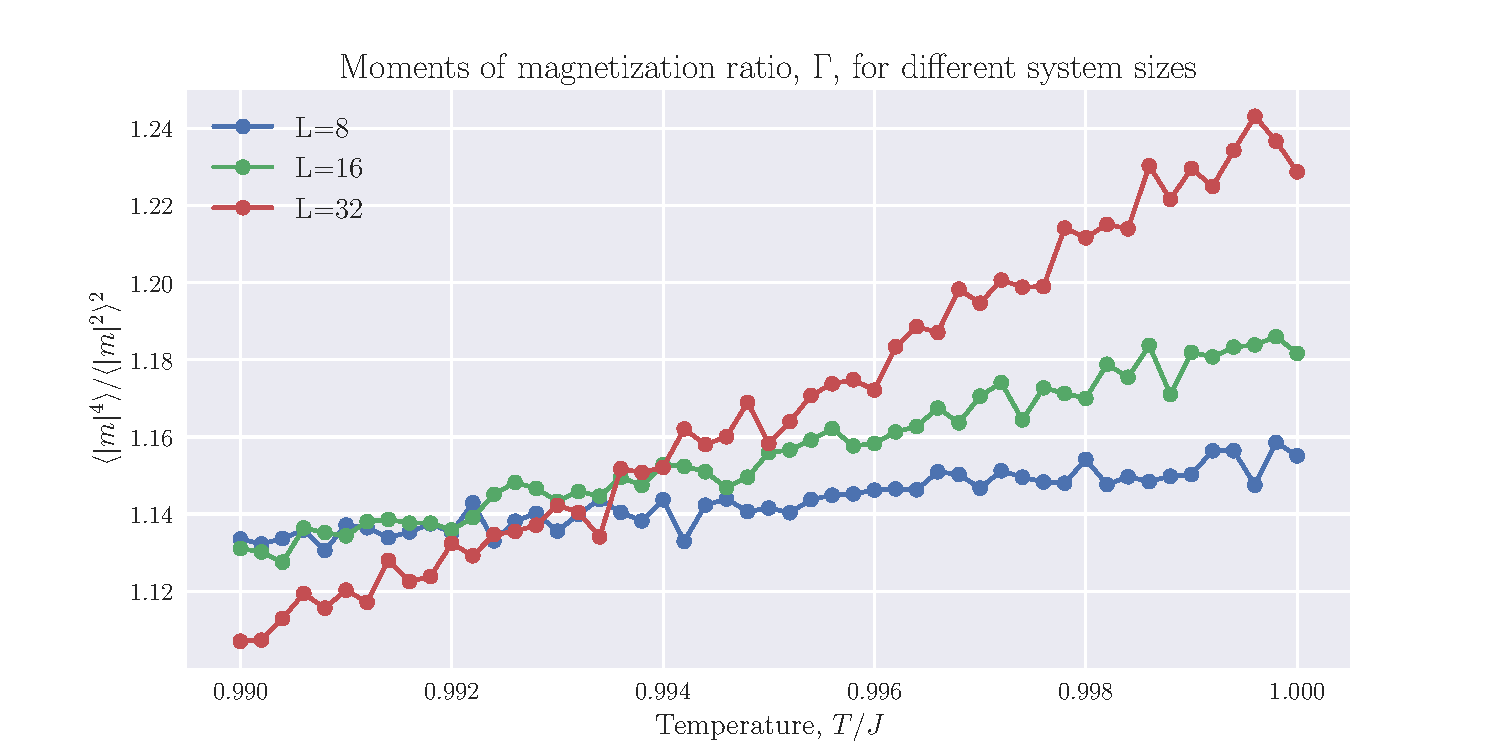
\includegraphics[width=0.7\linewidth]{gamma_curves_N51_dT001.pdf}
	\caption{Moments of magnetization for different system sizes near the region $T=0.995$ where we expect to find $T_c$.}
	\label{fig:gamma_dense}
\end{figure}

Instead, we assume that curves don't cross at a single point due to the phrasing of the task. There are a few possible reasons for non-overlapping curves that I may think of. One of these, is that we don't have an actual lattice spacing in our model, but have a Hamiltonian which considers neighbouring spins. However, the behaviour of the Hamiltonian under RG transformations may be affected, but it's hard to conclude, as we don't have any concrete expressions. 

Another peculiar fact, is that we actually scale the size of the system in these models, so we have $L^{-1}\to \frac{1}{2}L^{-1}$ when we go from e.g. $L=16$ to $L=32$. Setting $s=L$ to obtain $g(tL^{y_t})$ is then no longer possible, and expanding the function around $t=0$ may actually yield a factor $L$ in one of the constant terms, which means that $\Gamma$ is affected by $L$ at $t=0$. It may be that I've completely misunderstood how the finite size scaling works, but I don't see how we can set $s=L$ in our model. It may be that we should have used $s^{y_L}$, which could then yield some dependency on particular values of $L$. 

Next, we didn't take into account what $y_t$ is. I struggle to see how and why it should be a repuslive or attractive fixed point at all, but this may be a consequence of computing actual transformations which we haven't considered. In these actual transformations there could also be higher order terms contributing, which means that the general transformation relation $Q(s\{K\})\sim sQ(\{Ks^{y_k}\})$ would be invalid for our model. I'm also not entirely sure that $\Gamma$ itself should stay unscaled. Perhaps it should scale by some dimensionless quantity that is dependent of on the system size in some ways.  

As a final consideration, we never really took into account the behaviour of $\Gamma$ for $t\neq0$. For low values of $T$ we have $\Gamma\to1$ and for $T\to2$ we have $\Gamma\to2$. Perhaps an investigation and more thorough consideration of these limits could help solve the puzzle. But it's also possible that the answer simply is that $L$ is too low for crossing to take place.    


\end{document}
